\documentclass{salt}

% This document template was developed by the editors of /Semantics and
%  Pragmatics/ and minimally modified to work with the salt.cls document
%  class.

\usepackage{tikz, tikz-qtree}
\usepackage{gb4e-salt}
\usepackage{tipa}
\usepackage{enumerate}
\usepackage{graphicx}
% To generate the BibTeX logo
\newcommand{\BibTeX}{{\sc Bib}\TeX }

%=====================================================================
%========================= preamble material =========================

% Metadata for the PDF output. ASCII-only!
\pdfauthor{Anca Chereches, Neil Ashton, and David Lutz}
\pdftitle{Instructions for SALT 22 authors}
\pdfkeywords{SALT 22, proceedings, instructions}

% Optional short title inside square brackets, for the running headers.
% If no short title is given, no title appears in the headers.
\title[SALT 22 proceedings information]{Proceedings of SALT 22: \\ Information for contributors%
  \thanks{Thanks to the SALT 22 organizers, the LSA and eLanguage, the editorial and technical teams of \emph{Semantics and Pragmatics}, and the Department of Linguistics at Cornell University.}}

% Optional short author inside square brackets, for the running headers.
% If no short author is given, no authors print in the headers.
\author[Chereches, Ashton, and Lutz]{% As many authors as you like, each separated by \AND.
  \saltauthor{Anca Chereches \\ \institute{Cornell University}} \AND
  \saltauthor{Neil Ashton \\ \institute{Cornell University}} \AND
  \saltauthor{David Lutz \\ \institute{Cornell University}}%
}

%=====================================================================

\begin{document}

%=====================================================================
%============================ frontmatter ============================

\maketitle

%--------------------------------------------------------------------
% First page headers and page numbers
%
% the page number of the first page of this paper
\setcounter{page}{1}
% Create the first page headings.
% This needs to be issued *after* \maketitle.
%       {volume}{first page}{last page}{year}{not used}{not used}
\firstpageheadings{22}{1}{15}{2012}{}{}
%
%
%---------------------------------------------------------------------

\begin{abstract}  
  We describe the style guidelines and submission process for papers that will appear in the proceedings of SALT 22.
\end{abstract}

\begin{keywords}
  SALT 22, proceedings, instructions
\end{keywords}

\tableofcontents

\section{Introduction}\label{sec:introduction}

In this document, we describe the style guidelines and submission procedure for papers in the Proceedings of SALT 22. Extended discussions of the style guidelines and submission/publication procedure can be found in sections (\ref{sec:style-guidelines}) and (\ref{sec:submission-procedure}), respectively.  To summarize:

\begin{itemize}
  \item The submission deadline is \textbf{Wednesday, August 1 2012}.
  \item The page limit is \textbf{18 pages} for papers and posters, \textbf{24 pages} for invited speakers, both limits \textbf{excluding references}.
  \item We encourage authors to write using \LaTeX. Class and style files, as well as a template, accompany these instructions. We offer practical suggestions and usage examples in sections (\ref{sec:latex}) and (\ref{sec:examples}) respectively.  Those using other authoring software should consult the guidelines in section (\ref{sec:other-auth-softw}).
  \item Submissions should be  ``camera ready'', in \textbf{pdf format}, and submitted using the online submission system on the \href{http://www.elanguage.net/journals/index.php/salt}{SALT proceedings website}. Please do not send submissions via email.
  \item Questions and comments may be directed to \href{mailto:salt-mailbox@cornell.edu}{salt-mailbox@cornell.edu}.
\end{itemize}
  

\section{Style guidelines}\label{sec:style-guidelines}

We encourage authors to contacts us with any questions or concerns regarding formatting and abiding by the style guidelines. The easiest way to typeset your paper according to the SALT Proceedings guidelines is to use our \LaTeX{} template, which we provide in this bundle along with a number of helpful packages. If you choose to compose your paper using other authoring software (including word processors such as Microsoft Word and iWork's Pages), please follow the guidelines we provide in section (\ref{sec:other-auth-softw}).

\subsection{\LaTeX}\label{sec:latex}
We invite authors writing with \LaTeX{} to use the template provided with the SALT 22 bundle as the base for writing their papers. 

\subsubsection{\LaTeX{} class and style files}

The \LaTeX\ files in the SALT author bundle are derived from those of \emph{Semantics and Pragmatics}\footnote{\url{http://semprag.org}}, and we encourage authors to consult the S\&P author documentation for detailed information. The files in the bundle are:

\begin{description}
  \item[rights-form.pdf] \ This form must be filled out, signed by all authors, and returned to the editors.  No paper may be published unless we have signed rights forms from each of the paper's authors.
  \item[salt22-instructions.pdf]\  The current file, which advises on style guidelines and the submission process.
  \item[salt22-instructions.tex]\  The \verb+tex+ source file for this document.
  \item[salt22-template.tex]\  We encourage you to use this template source file as the skeleton of your paper. It loads the class file and illustrates all the basic commands you might need to structure a SALT submission. It does not load any additional packages that you might need for displaying numbered examples, trees, and so on. See section (\ref{sec:examples}) for examples of such extra functionality.
  \item[salt.cls] \ The SALT class file is responsible for the layout of your paper. The class file is loaded using the command \verb+\documentclass{salt}+, which is the first line in our template file \verb+salt22-template.tex+. The file \verb+salt.cls+ loads a number of useful packages, all of which should already be included in your \LaTeX{} distribution. Note that, should you need any of these packages, you will not have to load them again in your preamble: \verb+fontenc+, \verb+textcomp+, \verb+microtype+, \verb+natbib+, \verb+color+, \verb+hyperref+, \verb+amsmath+, \verb+ifpdf+, \verb+breakurl+, \verb+graphicx+, \verb+float+.
  \item[sp.bst]\ The bst file handles references using \BibTeX\ and is loaded automatically by \verb+salt.cls+ (so you do not need to call \verb+\bibliographystyle+ in your \verb+.tex+ document). This bibliography style file was developed by the technical team of \emph{Semantics and Pragmatics}, and we use it with their kind permission. Like the S\&P editors, we suggest you include doi and/or url information in your bibliography database entries.  Please consult section (3.4.2) of the S\&P author documentation\footnote{\url{http://semantics-online.org/sp/sp-latex.zip}} for information on the citation commands that the class file makes available.
   \item[supplementary-styles] This directory includes a selection of commonly used linguistics \LaTeX\ packages. We provide brief usage examples in section (\ref{sec:examples}). None of these packages is required or activated automatically by the \verb+salt.cls+ class file. Load them separately in your preamble using the command \verb+\usepackage{PackageName}+.\end{description}
   
Using our \LaTeX\ class is convenient because much of the formatting is automatic and streamlined. In our experience, there are only a few points that require extra attention: references to sources and examples, and formatting your list of references. These are discussed in the S\&P author documentation and we briefly describe them below.

\subsubsection{In-text citations}

How you cite a source should depend on how you are referring to it in context. You may be referring to the individual who authored a particular text or to the text itself. Examples of such contexts and what citation form to use follow below. 

\begin{description}
\item[Referring to the individual-as-author] For instance, ``\ldots was demonstrated by \pgcitet{Lewis-1973-counterfactuals}{74}'' or ``Following \citet{Lewis-1973-counterfactuals}, who showed that \ldots''. Note that the date (or a term such as \textit{to appear}, \textit{forthcoming}) is in parentheses, while the author is not.
\item[Referring to the work itself] In contexts such as ``For further discussion, see \pgcitealt{Lewis-1973-counterfactuals}{74}'' or ``The issue was first noticed in \citealt{Lewis-1973-counterfactuals}'', the date is not enclosed in parentheses. If the citation is meant to be parenthetical (e.g.  ``\ldots has been a controversial problem \citep{ccs2007, p2011}''), then the whole citation is enclosed in parentheses.
\end{description}

Additionally, SALT has guidelines for citing specific sections or page numbers. Conveniently, there are variants of the \verb+\cite+ command for almost any occasion. 

\begin{exe}
\item 
\begin{enumerate}
\item \verb+\citeauthor{p2011}+ $\Rightarrow$ \citeauthor{p2011} 
\item \verb+\citealt{p2011}+ $\Rightarrow$ \citealt{p2011} 
\item \verb+\citet{p2011}+ $\Rightarrow$ \citet{p2011} 
\item \verb+\citep{p2011}+ $\Rightarrow$ \citep{p2011}
\item \verb+\posscitet{p2011}+ $\Rightarrow$ \posscitet{p2011}
\item \verb+\possciteauthor{p2011}+ $\Rightarrow$ \possciteauthor{p2011} 
\item \verb+\pgposscitet{p2011}{7}+ $\Rightarrow$ \pgposscitet{p2011}{7}
\item \verb+\secposscitet{p2011}{4}+ $\Rightarrow$ \secposscitet{p2011}{4}
\item \verb+\pgcitealt{p2011}{7}+ $\Rightarrow$ \pgcitealt{p2011}{7}
\item \verb+\seccitealt{p2011}{4}+ $\Rightarrow$ \seccitealt{p2011}{4} 
\item \verb+\pgcitep{p2011}{7}+ $\Rightarrow$ \pgcitep{p2011}{7}
\item \verb+\seccitep{p2011}{4}+ $\Rightarrow$ \seccitep{p2011}{4} 
\item \verb+\pgcitet{p2011}{7}+ $\Rightarrow$ \pgcitet{p2011}{7} 
\item \verb+\seccitet{p2011}{4}+ $\Rightarrow$ \seccitet{p2011}{4}
\end{enumerate}
\end{exe}

We highly recommend using these commands for your in-text citations. They make future changes in formatting or spelling straightforward and help check that all your citations correspond to entries in the list of references.

\subsubsection{Examples}

The SALT author bundle provides \verb+gb4e-salt.sty+ for handling numbered examples according to the SALT guidelines (see section (\ref{gb4e}) for examples). However, you may use any other package you might prefer as long as the outcome is as described in section (\ref{sec:other-auth-softw}) and as illustrated in section (\ref{gb4e}).

Here we would like to note the most common editorial observations we have made so far.

\begin{exe}
\ex 
\begin{enumerate}
\item Example sentences in object language should end in appropriate punctuation.
\item In-text references to examples should be enclosed in parentheses. For example, we could be discussing the mundane example in (\ref{exe:sent}), the subexamples (\ref{exe:sents}a-c), or just (\ref{exe:sents}a,c) thus excluding (\ref{exe:sents}b). References to section numbers should be treated the same way.
\item Though surrounded by parentheses, in-text references to examples should not be considered parenthetical. For instance, instead of ``Example sentences can be quite short (\ref{exe:sent}).'' consider ``Example sentences can be quite short, as illustrated in (\ref{exe:sent}).'' or any alternative in a similar vein.
\end{enumerate}
\end{exe}

\subsubsection{List of references}

The SALT class file needs your bibliographic database \verb+my-references.bib+\footnote{Note that since we are using the \BibTeX\ program for bibliography management, you cannot simply embed your references at the end of the document using a \texttt{thebibliography} environment.} and the bibliography style file \verb+sp.bst+ (provided in this package) to allow you to include your list of references. The style file is loaded automatically, so you do not need the command \verb+\bibliographystyle{sp}+ in your \LaTeX\ source file. However, you do need to include the command \verb+\bibliography{my-references}+ (where \verb+my-references.bib+ is the name of your bibliography database file) after the main text and any appendices, but before the author addresses section.  

When compiling your \BibTeX\ database entries, please be mindful of the following style guidelines: 

\begin{itemize}
\item Journal and book titles must be given in full with initial letter of each major word capitalized (title case).
\item Check your \verb+pdf+ to make sure that journal titles, book titles, proper nouns and acronyms are properly capitalized. If they are not, you can preserve capitalization by enclosing the offending letters in curly braces in your \BibTeX\ entries. For example, ``Booktitle = \{Semantics and \{L\}inguistic \{T\}heory (\{SALT\}) 20\}'' from our very own \verb+salt22-instructions.bib+.
\item Page references must be given in full for all articles in books and journals.
\item Use full first names of authors or editors.
\item In case of multiple authorship, the names of all authors must be given.
\item When possible, provide the issue number and not just the volume number for a journal article.
\item Provide the doi number of a journal article whenever possible.  If the information is not directly available with the article, use the form at \href{http://crossref.org}{crossref.org} to find the doi.
\item For a conference proceedings title, use the name of the society and then put the meeting's acronym in parentheses.  Otherwise treat as a journal article. Do not include the words ``proceedings of the'' or ``papers from the''.  You need not list all the editors in full. This information can be difficult to come by.
\end{itemize}

\subsection{Other authoring software} \label{sec:other-auth-softw}
If you are using anything other than \LaTeX\ to typeset your paper, you will need to manually format your paper to correspond to the SALT style guidelines. Since the submission format is \textbf{pdf}, please keep in mind that the editors will not be able to modify any submission ourselves. Hence, it is the author's responsibility to submit a paper that conforms to these style guidelines.

\paragraph{General}
The article should be single-spaced, aligned both on the left and on the right. The font is Times New Roman, 12 pt. Other special formatting is addressed in what follows.

\paragraph{Margins}
The page should be 8.5 by 11 inches (standard US letter dimensions). The margins should be 1.5 inches for top, bottom, left, and right. Headers and footers should be within the margins, each 1 inch from the top and bottom of the page.

\paragraph{Headers and Footers} 
Both headers and footers use 10pt font.

Headers start on the second page of the document (the top of the first page is dedicated to title and abstract information). On even pages, headers include the last names of the authors, right justified; on odd pages, they include the title, optionally abbreviated, left justified, with no other special formatting.

Page numbers go in footers, centered, with no punctuation, starting on the second page. Page numbers will be assigned to each article after copyediting has been completed. On the first page only, the footer contains copyright information, justified left, as follows:
 
 \
 
 \hspace{-.25in}\footnotesize \copyright 2012 Author Last Names \normalsize
 
\paragraph{Footnotes}
Footnotes should use 10pt font size and should be separated from the main body by a small horizontal line (see the pdf files in this bundle for illustration). They should be numbered incrementally using Arabic numerals (with the exception of footnotes related to the title, authors, or abstract).

\paragraph{First page}
\subparagraph{First page header}
The first line on the first page should be the first page header, which should be justified left, 10pt font size, and should contain the following information:

\

\hspace{-.25in}\footnotesize Proceedings of SALT 22: XXX\textendash XXX, 2012 \normalsize

\

XXX should be replaced with your page numbers, once they have been assigned (after copyediting has been completed). The text ``Proceedings of SALT'' should ideally link to the following URL: \url{http://elanguage.net/journals/index.php/salt}.

\subparagraph{Title and author}
There are two empty lines (at 12 pt each) before the title. The title should be sized at 14 pt, bold, centered, in sentence case (only first word and proper nouns capitalized). Add an extra 12 pt empty line after the title, followed by the name of the author (12 pt, regular, centered) and, on a new line, the institution (12 pt, italics, centered). When the paper is co-authored, two authors may appear side-by-side, a third author appears centered below.

\subparagraph{Abstract and keywords}
The entire abstract paragraph should be indented 0.25 inches from the left margin and 0.25 inches from the right margin, aligned both on the left and the right side. Before and after the abstract paragraph there are two empty lines (12 pt). The abstract is written in 11 pt font.

As mentioned above, there are two empty lines (of 12 pt each) between the abstract and keywords. However, keywords are not indented; they are flush left. Keywords are also separated from the main body of the text by two empty lines, 12 pt each.


\paragraph{Main body}
The body of the article should be 12 pt Times New Roman, aligned both on the right and left side. Paragraphs are indented at 0.25 inches, with the exception of the first paragraph after a section heading, a figure, list, table, or anything that might interrupt the main body text.

\subparagraph{Sections}

Sections are given running numbers, subsections given running sub-numbers separated from the main section number by a period. Section and subsection titles (and their numbers) are set in bold face with sizing identical to body text. The numbers are set flush left, and the titles are separated from the numbers by a space of 1 em. There is a 10 pt space after the title and a 18 pt space before the title. The first paragraph after a title is not indented.

\subparagraph{Examples}

Example sentences are given running numbers, with numbers in round parentheses flush left. Use Arabic numerals inside the main text and lowercase Roman numerals inside footnotes. There is a 7pt space before and after a set of example sentences, separating them from the main text. Paragraph spacing inside the set of example sentences should be adjusted as well: ``Spacing before line'' to 2pt and ``Spacing after line'' to 0pt. We are assuming that spacing between lines in the main text is 0pt. Example sentences are indented to a depth of 0.4 inches. See the examples in section (\ref{gb4e}).

Subexamples are given lowercase alphabetical letters followed by a period, indented to 0.4 inches to align with example sentences. Equations are given numbers in the same sequence as example sentences and spaced identically to those. References to examples are given within parentheses without internal punctuation, e.g. (\ref{raw}), (\ref{embedded}). See section (\ref{gb4e}) for formatting examples.

Example sentences in object language should be ended with proper punctuation, such as periods.

\subparagraph{Figures, tables}

Figures and tables are set at the top of the page, delineated by a preceding and a following horizontal line which span the width of the text body. A 5 pt break precedes and follows each line. An additional 10 pt break separates the bottom line from the main body text.

The caption of a figure or a table is separated from its body by a 10 pt break. Captions are given a boldface label, indented to 0.15 inches, that identifies its type and assigns it a running number (e.g. ``\textbf{Figure 1}'', ``\textbf{Table 1}''). Figures and tables have separate running number counts. The caption itself is set in the main body font, indented to 0.85 inches.

\begin{figure}
\includegraphics[width=5.5in]{figure.png}
\caption{A summary of the submission and publication process.}
\end{figure}

\paragraph{In-text Citations}\label{sec:citations}

We adopt the guidelines of \emph{Semantics and Pragmatics} for in-text citations, which can be found in their author guidelines.\footnote{\url{http://semantics-online.org/sp/sp-latex.zip}}  They are also repeated here with trivial modifications:
\begin{itemize}
\item Page numbers are separated from the year by a nonbreaking space: \pgcitep{Lewis-1973-counterfactuals}{74}.
\item Section and chapter numbers are separated from the year by a   non-breaking space and coded with \S: \seccitep{p2011}{4}.
\item References to articles are given without parentheses: \citealt{Lewis-1973-counterfactuals}, \pgcitealt{Lewis-1973-counterfactuals}{74}.
\item References to an individual-as-author-of-a-text are given with the name followed by the year and other material inside parentheses: \citet{Lewis-1973-counterfactuals}, \pgcitet{Lewis-1973-counterfactuals}{74}.
\item Possessive marking is on the name only: \posscitet{p2011}, \secposscitet{p2011}{4}.
\item Parenthetical references to articles do not contain parentheses of their own:  \citep{p2011}, \seccitep{p2011}{4}.
\end{itemize}


\paragraph{References}

References should adhere to the guidelines set forth in the S\&P author documentation, section (3.5.2), and repeated here: 

\begin{itemize}
\item Use full first names of authors or editors.
\item In case of multiple authorship, the names of all authors must be given.
\item Journal and book titles must be given in full with initial letter of each major word capitalized.
\item Page references must be given in full for all articles in books and journals.
\item When possible, provide the issue number and not just the volume number for a journal article.
\item Provide the doi number of a journal article whenever possible.  If the information is not directly available with the article, use the form at \href{http://crossref.org}{crossref.org} to find the doi.
\item For a conference proceedings title, use the name of the society and then put the meeting's acronym in parentheses.  Otherwise treat as a journal article. Do not include the words ``proceedings of the'' or ``papers from the''.  You need not list all the editors in full. This information can be difficult to come by.
\end{itemize}

References should be listed in alphabetical order by the authors' last names. See the references in this document for an example of the bibliography style produced by \verb+sp.bst+. If you are not using \LaTeX, we ask that you attempt to replicate this style as closely as possible. 

\paragraph{Backmatter}

The names and addresses of all authors are listed at the end of the document, following the bibliography. See the end of this document for an example of the appropriate format for addresses.


\section{Submission and publication  procedure}\label{sec:submission-procedure}

The proceedings of SALT are published by \href{http://www.elanguage.net}{eLanguage}, the electronic publishing platform of the LSA.  This section is a step-by-step description of the submission and publication procedure for authors.  

\begin{enumerate}[1. ]
  \item Fill out, sign, and return the rights form included with this bundle.  Co-authors may submit a single form signed by all authors, separate forms for each author, or a combination.  Information about how to submit the form is given on the form.
  \item Register/Log in to the SALT website
  \begin{itemize}
    \item Go to the SALT proceedings website at  \url{http://elanguage.net/journals/index.php/salt}.
    \item If you're not already registered with an eLanguage journal, please register.  Make sure to select ``Register as: Author'' near the bottom of the screen.
    \end{itemize}
  \item Submit your manuscript
    \begin{itemize}
      \item Once you are registered and logged in, go to your ``Author''  page (under ``User Home'') and start a new submission.
      \item Follow the five-step submission process.  Please note that an abstract is required, and keywords are recommended, as they increase your work's visibility to search engines.
      \item The submission file should be in pdf format.
      \item Consider including your results, data, etc. as a supplementary file in some archive format (.zip, .tar.gz., etc.).  This file will be made available to readers.
    \end{itemize}
    \item Complete copyediting
      \begin{itemize} 
      \item The editors will read your paper and check for typographical and layout errors and adherence to these style guidelines.  If problems are noted, you will receive an email asking you to submit a corrected pdf.
      \end{itemize}
     \item Add page numbers 
       \begin{itemize}
         \item Once copyediting is completed, your paper will have page numbers assigned.  Please add the assigned page numbers to the header on the first page as well as to the footer of every page other than the first.
       \end{itemize}  
     \item Publication 
       \begin{itemize}
         \item After page numbers have been added, your paper will appear on the SALT website, and the corresponding author will receive an email notification of publication.
        \end{itemize}
       
\end{enumerate}
     

\section{Examples}\label{sec:examples}

Standard \LaTeX\ distributions include a number of packages which are useful for the working linguist. The SALT style sheet also includes a number of macros\footnote{These macros and examples come respectively from the \texttt{sp-latex} package and its documentation. We are grateful to the authors for both.} designed to accommodate semanticists' typical typographical needs. We include here illustrative examples of these macros and certain key \LaTeX\ packages.\footnote{To include a package, add a package declaration of the form ``\texttt{$\backslash$usepackage\{package name\}}'' in the preamble of your document.}

\subsection{Useful macros}

A macro for denotation function brackets, \verb+\sv+, is provided. To typeset \sv{beekeeper}, for example, use \verb+\sv{\text{beekeeper}}+. Note that \verb+\sv+ creates a math environment but does not itself need to be used in a math environment.

Incorrect spacing will result if the character ``:'' is used to typeset the colon in logical and set-theoretic expressions. The macro \verb+\co+ (in math environment) produces the appropriate result.

\begin{quote}
\small
\begin{verbatim}
$\forall x\co x \in D \dots$
\end{verbatim}
\end{quote}

\begin{quote}
$\forall x\co x \in D \dots$
\end{quote}

The \verb+\http+ and \verb+\email+ macros convert a string into a clickable link, allowing you to insert clickable web and email addresses into your document. For example, \verb+\http{elanguage.net}+ produces \http{elanguage.net}, \verb+\email{+\texttt{salt-mailbox@ cornell.edu}\verb+}+ produces \email{salt-mailbox@cornell.edu}.


\subsection{\texttt{gb4e-salt}} \label{gb4e}

The \verb+gb4e-salt+ package is variant of the \verb+gb4e+ set of macros\footnote{\http{http://www.ctan.org/tex-archive/macros/latex/contrib/gb4e/}} designed to simplify the typesetting of numbered examples, glossed and otherwise, according to the SALT formatting guidelines.

A batch of examples is wrapped in the \verb+exe+ environment, with each example introduced by \verb+\ex+. Embedded sub-batches of examples are introduced by the \verb+xlist+ environment. Grammaticality judgment labels are optionally added in square brackets after the \verb+\ex+ command, in which case the example is supplied to \verb+\ex+ in curly braces as an argument.

Here is an example:

\begin{quote}
\small
\begin{verbatim}
\begin{exe}
    \ex This is a sentence.
    \ex[]{This is also a sentence.}
    \ex[*]{This bad a sentence is.}
    \ex[??]{A questionable sentence this is.}
    \ex
        \begin{xlist}
            \ex This is embedded.
            \ex[]{So is this.}
            \ex[*]{Is so this.}
        \end{xlist}
\end{exe}
\end{verbatim}
\end{quote}

This produces:

\begin{exe}
    \ex This is a sentence.
    \label{exe:sent}
    \ex[]{This is also a sentence.}\label{raw}
    \ex[*]{This bad a sentence is.}
    \ex[??]{A questionable sentence this is.}
    \ex \label{exe:sents}
        \begin{xlist}
        
            \ex This is embedded.\label{embedded}
            \ex[]{So is this.}
            \ex[*]{Is so this.}
        \end{xlist}
\end{exe}

Examples produced in this way are assigned running numbers. When specific numbers are called for (as with cited examples), the \verb+\exi+ command is used.

\begin{quote}
\footnotesize
\begin{verbatim}
\begin{exe}
    \exi{(14)} If Carl is at the party, then Lenny
                   must be at the party. \\
               Carl is at the party. \\
               So: Lenny is at the party.
    \exi{(2)} I am NOT NOT NOT letting someone take 
                   out part of my liver!
    \exi{(39)}[*]{Her$_i$ father loves everyone's$_i$ mother}
\end{exe}
\end{verbatim}
\end{quote}


\ldots repeated here from \pgcitealt{vfg2010}{367}, 
    \pgcitealt{p2011}{655}, and \pgcitealt{ccs2007}{146}:
\begin{exe}
    \exi{(14)} If Carl is at the party, then Lenny 
                   must be at the party. \\
               Carl is at the party. \\
               So: Lenny is at the party.
    \exi{(2)} I am NOT NOT NOT letting someone take 
                   out part of my liver!
    \exi{(39)}[*]{Her$_i$ father loves everyone's$_i$ mother}
\end{exe}

\verb+gb4e-salt+ also offers macros for glossed examples. A glossed example is an \verb+ex+ example containing up to two additional commands: \verb+\gll+, which introduces a sentence-gloss pair, and \verb+\glt+, which introduces a free translation.

\begin{quote}
\small
\begin{verbatim}
\begin{exe}
    \ex \gll Ho inghiottito un ape. \\
             have swallowed a bee \\
        \glt `I swallowed a bee.'
    \ex \gll Lo ho inghiottito. \\
             it have swallowed \\
\end{exe}
\end{verbatim}
\end{quote}

\begin{exe}
    \ex \gll Ho inghiottito un ape. \\
             have swallowed a bee \\
        \glt `I swallowed a bee.'
    \ex \gll Lo ho inghiottito. \\
             it have swallowed \\
\end{exe}


Note that glosses are matched word by word, with words counted by whitespace. Multi-word glosses must be wrapped in curly braces, and empty elements must be matched in the gloss by empty pairs of curly braces.

\begin{quote}
\small
\begin{verbatim}
\begin{exe}
    \ex \gll zum Imker \\
             {to the} beekeeper \\
    \ex \gll ?`Qu\'e$_i$ ella dijo $t_i$ a \'el? \\
             what she said {} to him \\
\end{exe}
\end{verbatim}
\end{quote}

\begin{exe}
    \ex \gll zum Imker \\
             {to the} beekeeper \\
    \ex \gll ?`Qu\'e$_i$ ella dijo $t_i$ a \'el? \\
             what she said {} to him \\
\end{exe}


\subsection{\texttt{tipa}}

Symbols from the International Phonetic Alphabet can be added to \LaTeX{} documents by means of the \texttt{tipa} package.

IPA symbols can be entered in one of two ways. They can first of all be entered as commands in the ordinary text environment, like so:

\begin{quote}
\small
\begin{verbatim}
[\textsecstress\textepsilon kspl\textschwa
\textprimstress ne\textsci\textesh\textschwa n]
\end{verbatim}
\end{quote}

Which produces:

\begin{quote}
[\textsecstress\textepsilon kspl\textschwa
\textprimstress ne\textsci\textesh\textschwa n]
\end{quote}

Alternatively, IPA characters can be entered as ``shortcut characters'' in a special \verb+tipa+ environment. A number of such environments are available. Each of the following produce the same string of characters as the above:

\begin{quote}
\small
\begin{verbatim}
\textipa{[""Ekspl@"neIS@n]}
{\tipaencoding [""Ekspl@"neIS@n]}
\begin{IPA}
    [""Ekspl@"neIS@n]
\end{IPA}
\end{verbatim}
\end{quote}

The two encodings are not strictly identical, and the latter is in fact superior for most purposes. The special \verb+tipa+ environment enables automatic kerning between characters, producing a more attractive result for strings of IPA symbols. Note, for example, the typographical differences between the following examples from the \verb+tipa+ manual.

\begin{quote}
\begin{verbatim}
v\textturnv v w\textsca w y\textturny y [\textesh]
\end{verbatim}
\end{quote}

\begin{quote}
v\textturnv v w\textsca w y\textturny y [\textesh]
\end{quote}

\begin{quote}
\begin{verbatim}
\textipa{v2v w\textsca w yLy [S]}
\end{verbatim}
\end{quote}

\begin{quote}
\textipa{v2v w\textsca w yLy [S]}
\end{quote}

For this reason, as well as the obvious convenience of the ``shortcut'' input method, the \verb+tipa+ environment is the preferred method of entering IPA transcriptions.

An annotated list of \verb+tipa+ commands and shortcut characters for IPA symbols can be found in the TIPA manual.\footnote{\http{ftp://ftp.dante.de/tex-archive/fonts/tipa/tipaman.pdf}}


\subsection{\texttt{tikz-qtree}}

David Chiang's \verb+tikz-qtree+ package provides macros for drawing trees. It combines the bracket notation syntax of Alexis Dimitriadis' Qtree package\footnote{\http{http://www.ling.upenn.edu/advice/latex/qtree/}} with the graphics macros of TikZ.\footnote{\http{http://sourceforge.net/projects/pgf/}}

A simple tree is written like so:

\begin{quote}
\small
\begin{verbatim}
\Tree [.S [.NP this ]
          [.VP is
               [.NP {a tree} ] ] ]
\end{verbatim}
\end{quote}

Which produces a tree like this:

\begin{center}
\Tree [.S [.NP this ]
          [.VP is
               [.NP {a tree} ] ] ]
\end{center}

The TikZ package provides various options and features useful for linguists, most of which require the tree to be wrapped in the \verb+tikzpicture+ environment. The vertical distance between parent and child nodes can be set with the \verb+level distance+ option and the horizontal distance between sisters by \verb+sibling distance+, for example:

\begin{quote}
\small
\begin{verbatim}
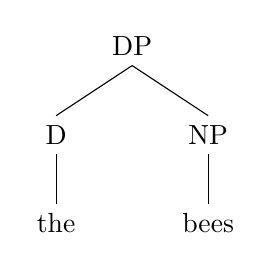
\begin{tikzpicture}[level distance = 32pt, sibling distance = 32pt]
\Tree [.DP [.D the ] [.NP bees ] ]
\end{tikzpicture}
\end{verbatim}
\end{quote}

\begin{center}
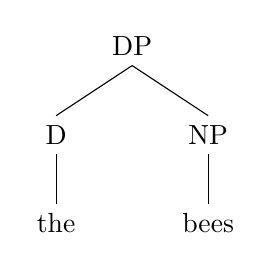
\begin{tikzpicture}[level distance = 32pt, sibling distance = 32pt]
    \Tree [.DP [.D the ] [.NP bees ] ]
\end{tikzpicture}
\end{center}

Arrows to and from nodes can be drawn with the help of the combination of the \texttt{node} command, which allows you to assign identifying names to nodes, and the transparently named \texttt{draw} command.

\begin{quote}
\footnotesize
\begin{verbatim}
\begin{tikzpicture}[level distance = 24pt, sibling distance = 24pt]
\Tree [.CP [.DP$_i$ \node(wh){what}; ]
           [.C$'$ [.I$_j$+C did ]
                  [.IP [.DP$_k$ I ]
                       [.I$'$ $t_j$
                              [.VP $t_k$
                                   [.V$'$ eat
                                          \node(base){$t_i$}; ] ] ] ] ] ]
\draw[semithick,->] (base) ..
    controls +(south west:3) and +(south:3)
    .. (wh);
\end{tikzpicture}
\end{verbatim}
\end{quote}

\begin{center}
\begin{tikzpicture}[level distance = 24pt, sibling distance = 24pt]
\Tree [.CP [.DP$_i$ \node(wh){what}; ]
		   [.C$'$ [.I$_j$+C did ]
		   		  [.IP [.DP$_k$ I ]
				  	   [.I$'$ $t_j$
					   		  [.VP $t_k$
							  	   [.V$'$ eat
								   		  \node(base){$t_i$}; ] ] ] ] ] ]
\draw[semithick,->] (base) ..
    controls
        +(south west:3)
        and +(south:3)
    .. (wh);
\end{tikzpicture}
\end{center}

A roof can be drawn over a node to cover irrelevant structure like so:


\begin{quote}
\small
\begin{verbatim}
\Tree [.DP [.NP \edge[roof]; {obviously way too complex
                              to properly parse noun phrase} ] ]
\end{verbatim}
\end{quote}

\begin{center}
\Tree [.DP [.D an ]
           [.NP \edge[roof]; {obviously way too complex
                              to properly parse noun phrase} ] ]
\end{center}

The further possibilities afforded by TikZ are too numerous to cover in any detail here, and the curious linguist is referred to the \texttt{tikz-qtree} documentation for details.\footnote{\texttt{\http{http://www.ctan.org/tex-archive/graphics/pgf/contrib/tikz-qtree/}}}
                     



%=====================================================================

\bibliography{salt22-instructions}

%=====================================================================

\begin{addresses}
  \begin{address}
    Anca Chereches \\
    203 Morrill Hall \\
    Cornell University \\
    Ithaca, NY 14850 \\
    \email{ac872@cornell.edu}
  \end{address}

  \begin{address}
    Neil Ashton \\
    203 Morrill Hall \\
    Cornell University \\
    Ithaca, NY 14850 \\
    \email{nma38@cornell.edu}
  \end{address}

  \begin{address}
    David Lutz \\
    203 Morrill Hall \\
    Cornell University \\
    Ithaca, NY 14850 \\
    \email{del82@cornell.edu}
  \end{address}

\end{addresses}

%=====================================================================

\end{document}


